\subsection{Интегрирование}
\label{sec:partint} 

\subsubsection{Формула Гаусса--Остроградского}

Формула Гаусса--Остроградского, связывающая
интегрирование по объёму $E$ с интегрированием по границе этого объёма $\Gamma$,
для векторного поля $\vec v$ имеет вид
\begin{equation}
\label{eq:partint_div}
\arint{\nabla\cdot\vec v}{E}{\vec x} = \arint{v_n}{\Gamma}{s},
\end{equation}
где $\vec n$ -- внешняя по отношению к области $E$ нормаль.
Смысл этой формулы можно проиллюстрировать на одномерном примере.
Пусть одномерное векторное поле $v_x = f(x)$ на отрезке $E = [a, b]$ задано
функцией, представленной на \figref{fig:div1d}.
\begin{figure}[h!]
\centering
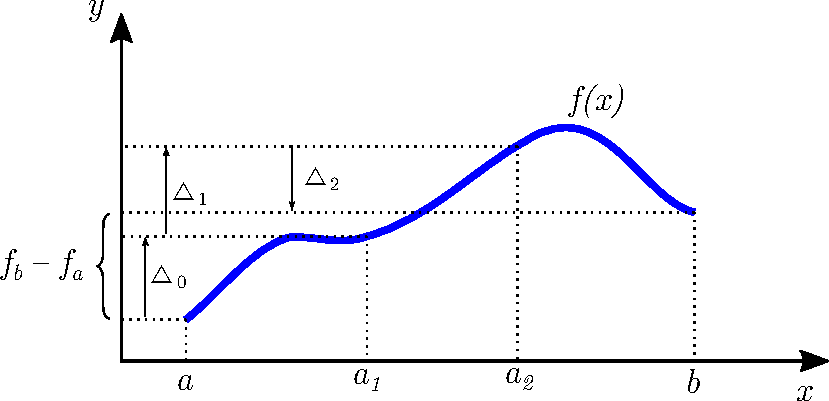
\includegraphics[width=0.6\linewidth]{div1d.pdf}
\caption{Формула Гаусса-Остроградского в одномерном случае}
\label{fig:div1d}
\end{figure}
Разобъем область на $N=3$ равномерных подобласти длины $h$. Тогда
расписывая интеграл как сумму, а производную через конечную разность, получим
$$
\arint{\dfr{f}{x}}{E}{x} \approx \sum_{i=0}^{2} h \left(\dfr{f}{x}\right)_{i+\tfrac12}
\approx\sum_{i=0}^{2}(f_{i+1} - f_{i})
= \triangle_0 + \triangle_1 + \triangle_2 = f_b - f_a.
$$
Очевидно что, при устремлении $N\to\infty$ правая часть предыдущего выражения не изменится.
То есть, сумма всех изменений функции в области есть изменение функции по её границам:
$$
\int\limits_{a}^{b}\dfr{f}{x}\,dx = f(b) - f(a).
$$
А формула \cref{eq:partint_div} -- есть многомерное обобщение этого выражения.

\subsubsection{Интегрирование по частям}

Подставив в \cref{eq:partint_div} $\vec v = f\vec u$, где $f$ -- некоторая скалярная функция, и 
расписав дивергенцию в виде
$$\nabla\cdot(f\vec u) = f\nabla\vec u + \vec u \cdot \nabla f$$
получим формулу интегрирования по частям
\begin{equation}
\label{eq:partint}
\arint{\vec u \cdot \nabla f}{E}{\vec x} = \arint{f u_n}{\Gamma}{s} - \arint{f\nabla\cdot \vec u}{E}{\vec x}
\end{equation}
Распишем некоторые частные случаи для формулы \cref{eq:partint}.
Для $\vec u = (n_x, 0, 0)$ получим
\begin{equation}
\label{eq:partint_ugrad_}
\arint{\dfr{f}{x}}{E}{\vec x} = \arint{f \cos(\vecangle{n}{x})}{\Gamma}{s}
\end{equation}
При $\vec u = \nabla g$
\begin{equation}
\label{eq:partint_laplace_fg}
\arint{f\left(\nabla^2 g \right)}{E}{\vec x} = \arint{f\dfr{g}{n}}{\Gamma}{s} - \arint{\nabla f \cdot \nabla g}{E}{\vec x}
\end{equation}
При $f=1$ и $\vec u = \nabla g$
\begin{equation}
\label{eq:partint_laplace}
\arint{\nabla^2 g}{E}{\vec x} = \arint{\dfr{g}{n}}{\Gamma}{s}
\end{equation}
